\chapter{Comparison with Other Results}

We're not doing this in a vacuum.

\section{Monophoton}

\section{Monojet / Mono-$Z$}

\section{Direct Detection}

We show the results in Fig.~\ref{fig:limits_direct}.

\begin{figure}[htbp]
  \centering
    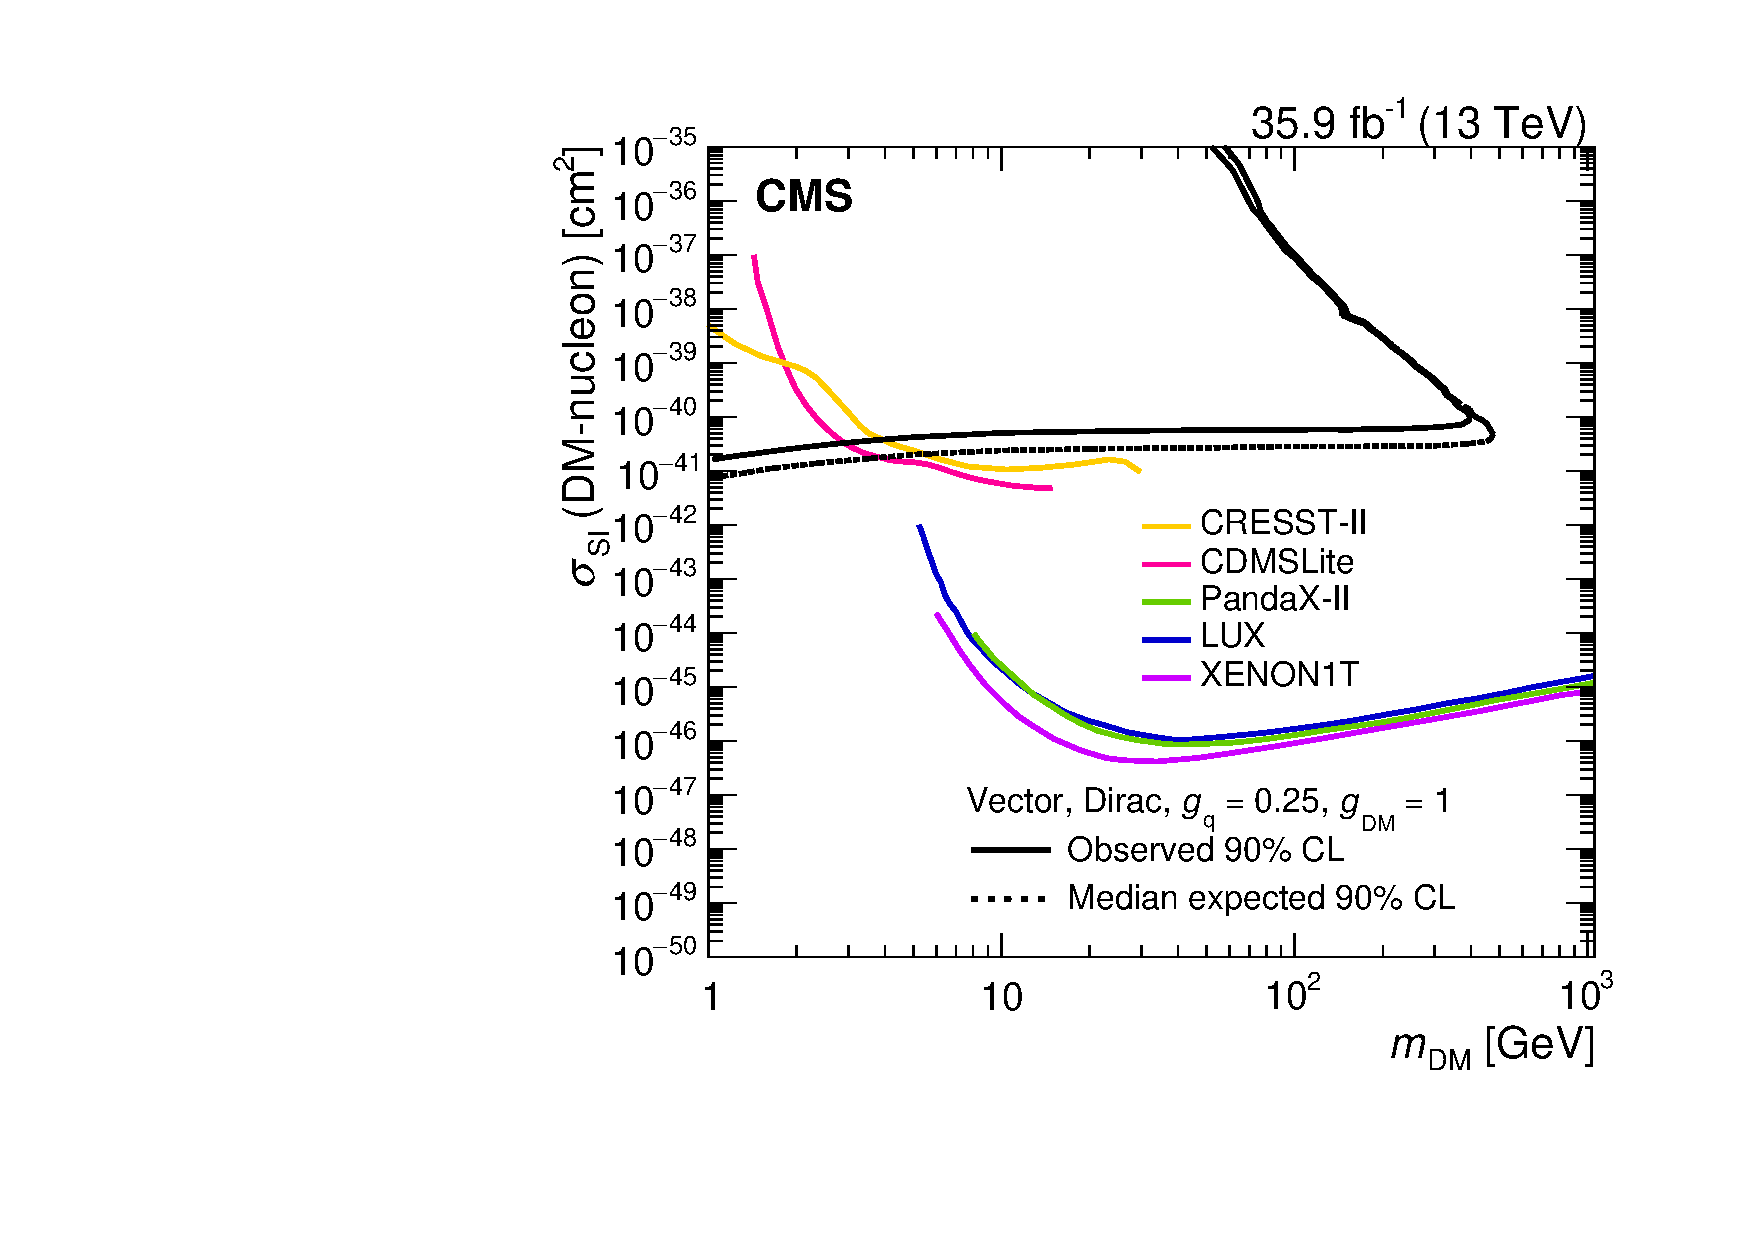
\includegraphics[width=0.48\linewidth]{Impact/Figures/limits_direct.pdf}
    \caption{
      The 90\% \CL\ exclusion limits on the $\chi$--nucleon spin-independent scattering cross sections involving the vector operator as a function of the \mdm.
      Simplified model DM parameters of $\gq=0.25$ and $\gDM=1$ are assumed.
      The region to the upper left of the contour is excluded. 
      On the plots, the median expected 90\% \CL\ curve overlaps the observed 90\% \CL\ curve.
      Also shown are corresponding exclusion contours, where regions above the curves are excluded, from the recent results by the CDMSLite~\cite{Agnese:2015nto}, LUX~\cite{Akerib:2016vxi}, PandaX-II~\cite{Cui:2017}, XENON1T~\cite{Aprile:2018}, and CRESST-II~\cite{Angloher:2015ewa}.
    }
    \label{fig:limits_direct}
\end{figure}

\section{Indirect Detection}

We show the results in Fig.~\ref{fig:limits_indirect}.

\begin{figure}[htbp]
  \centering
    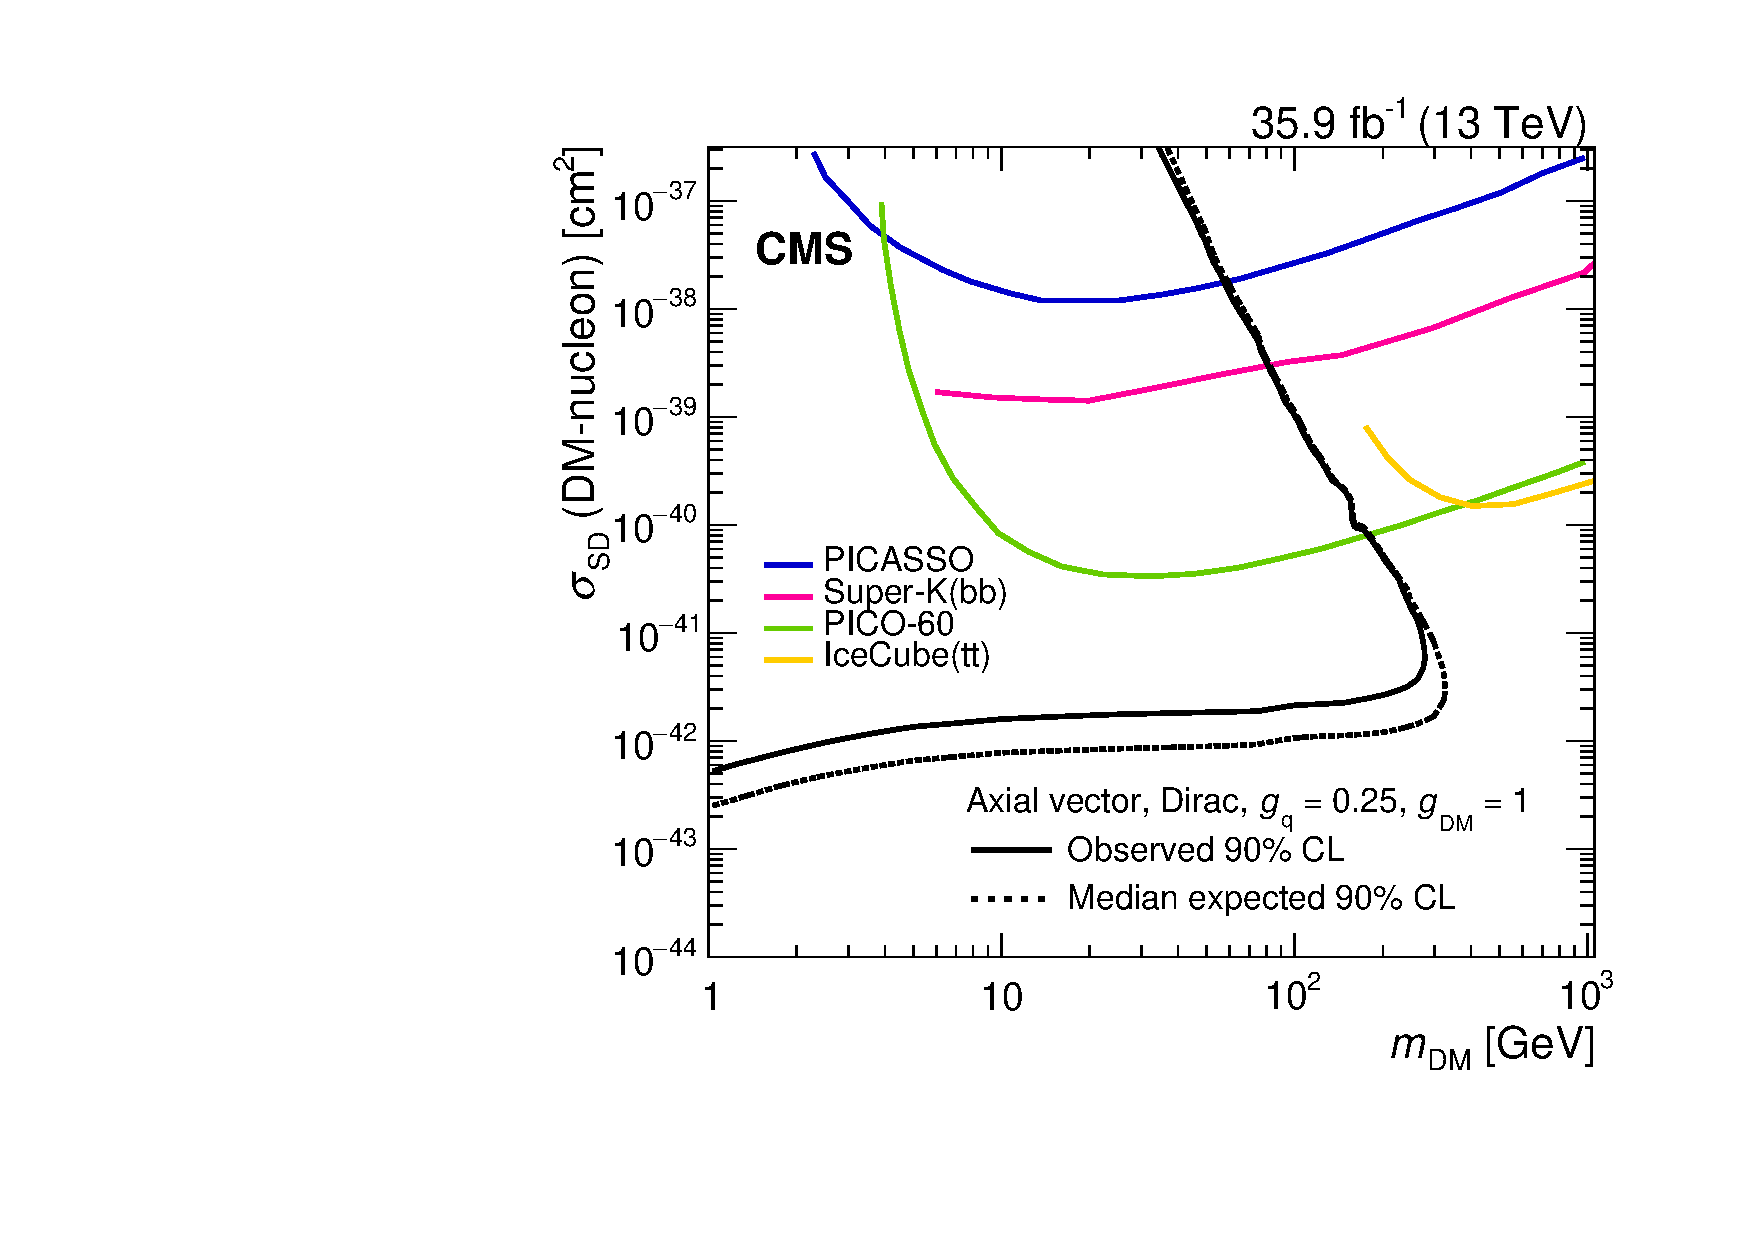
\includegraphics[width=0.48\linewidth]{Impact/Figures/limits_indirect.pdf}
    \caption{
      The 90\% \CL\ exclusion limits on the $\chi$--nucleon spin-dependent scattering cross sections involving the axial-vector operator as a function of the \mdm.
      Simplified model DM parameters of $\gq=0.25$ and $\gDM=1$ are assumed.
      The region to the upper left of the contour is excluded. 
      On the plots, the median expected 90\% \CL\ curve overlaps the observed 90\% \CL\ curve.
      Also shown are corresponding exclusion contours, where regions above the curves are excluded, from the recent results by the PICO-60~\cite{Amole:2017dex}, IceCube~\cite{Aartsen:2016exj}, PICASSO~\cite{Behnke:2016lsk} and Super-Kamiokande~\cite{Choi:2015ara} Collaborations.
    }
    \label{fig:limits_indirect}
\end{figure}
